\documentclass[12pt,a4paper]{article}
\usepackage[T1]{fontenc}
\usepackage[utf8]{inputenc}
\usepackage{newtxtext,newtxmath}
\usepackage[margin=30mm]{geometry}
\usepackage{microtype,booktabs,graphicx,amsmath,array,longtable}
\usepackage[authoryear,round,longnamesfirst]{natbib}
\usepackage{caption,placeins,fancyhdr,xurl,float}
\usepackage[hidelinks]{hyperref}
\hypersetup{pdftitle={The Index Effect in Sweden: A Replication and Extension of Greenwood and Sammon (2025)},pdfauthor={Alexander Fox and Ludvig Pauli Uvang},pdfsubject={Revised research working draft; AI-generated text for author review},pdfkeywords={OMXSB, Greenwood and Sammon, index effect, replication, event study}}
\captionsetup{font=small,labelfont=bf,justification=raggedright,singlelinecheck=false}
\setlength{\parindent}{1.2em}
\setlength{\parskip}{3pt}
\setlength{\emergencystretch}{2em}
\clubpenalty=10000
\widowpenalty=10000
\displaywidowpenalty=10000
\renewcommand{\baselinestretch}{1.02}
\pagestyle{fancy}\fancyhf{}\fancyfoot[C]{\thepage}
\fancyhead[L]{\small The Index Effect in Sweden}
\fancyhead[R]{\small Research draft}
\renewcommand{\headrulewidth}{0pt}
\setlength{\headheight}{15pt}
\begin{document}
\begin{titlepage}
\centering
\vspace*{20mm}
{\LARGE\bfseries The Index Effect in Sweden\par}
\vspace{8mm}
{\large A Replication and Extension of\par Greenwood and Sammon (2025)\par}
\vspace{16mm}
{\large Alexander Fox\par Ludvig Pauli Uväng\par}
\vspace{12mm}
Bachelor thesis research draft\par
Stockholm School of Economics\par
BE451 Degree Project in Finance\par
Autumn 2026\par
\vspace{10mm}
Tutor: Michael Klug\par
Examiner: Riccardo Sabbatucci\par
\vfill
\begin{minipage}{.88\textwidth}\small
Revised 12 November 2026. This is AI-generated research text for author review, not a submission version. The course prohibits AI directly writing the submitted thesis. Appendix~\ref{app:audit} gives the disclosure and verification status. Final submission requires author-written prose and the official cover template with verified student details.
\end{minipage}
\end{titlepage}
\thispagestyle{plain}
\begin{center}\large\bfseries The Index Effect in Sweden\end{center}
\begin{abstract}
We ask whether the disappearing index effect documented by Greenwood and Sammon (2025) also appears in Sweden, and what kind of return remains. Around OMX Stockholm Benchmark changes from July 2007 through June 2026, additions earn 2.15\% over the later decade, with a 95\% interval of [1.01\%, 3.39\%]. The latest five-year estimate is less precise. Covered benchmark-linked funds buy 1.03\% of shares outstanding on the matched later sample, and trading becomes more concentrated immediately before implementation. The positive addition association survives separately reported return exclusions and exceeds a size-screened comparison after correcting its control timing. Its historical decline is concentrated after a common initial seven-day window, while announcement lead times shorten. On a fixed later cohort, cumulative returns remain positive through twenty trading days after implementation. In a selected share-class sample, both the affected and sister classes move substantially, with an imprecise relative difference. The evidence supports a remaining later-decade addition association and identifies its trading and timing counterparts. It does not isolate a causal price response to index-fund demand. Changing holdings coverage particularly limits historical multiplier comparisons.
\end{abstract}
\noindent\textbf{Keywords:} index effect; replication; passive investing; reconstitution; fund holdings.\par
\newpage
\section{Introduction}

The growth of index investing creates a simple expectation: when more capital follows an index, changes in its membership should generate larger purchases and sales. Yet \citet{greenwood2025} document a striking development in the United States. Average returns around additions to the S\&P 500 fell from 7.4 \% in the 1990s to less than 1 \% in their latest decade, despite the expansion of index investing. Their study asks how markets have become able to accommodate these trades with a smaller price response. This thesis takes that question to Sweden.

We ask whether the disappearing index effect also appears around changes in the OMX Stockholm Benchmark Index (OMXSB), and what reported fund trading and the subsequent return pattern reveal about the association that remains. Our main finding is that later-decade additions continue to earn positive average market-adjusted returns. Their mean is 2.15 \% during 2017--2026. The historical pattern is nevertheless uneven, and the latest five-year estimate is less precise. Sweden therefore provides evidence of a positive later-period addition association without establishing that the effect is stable, permanent or caused by index membership.

The setting allows us to connect this return comparison to two features of the Swedish market. First, OMXSB changes occur in scheduled reviews, with several securities sharing an announcement and implementation date. The index selects securities using trading activity and industry representation, rather than a single market-capitalization boundary. Both the composition of additions and the time between announcement and implementation can consequently matter for measured returns. Second, Swedish companies often have more than one listed share class. When one class changes index status while another retains its status, their relative performance provides an additional perspective on whether the return movement is concentrated in the affected security or shared within the firm.

Our event register contains 536 changes across 39 reviews from July 2007 through June 2026. After return-data requirements and the stated event exclusions, the principal sample contains 256 additions and 215 deletions. Following the anchor study's event-window approach, we examine announcement returns, implementation returns and the interval from the day before announcement through the day after implementation. Our primary cumulative abnormal return is the sum of daily stock returns less the OMXSB gross-index return. We combine these returns with dated fund classifications and reported holdings, and compare the commercial holdings measure with regulatory fund reports. Inference clusters events by review because their dates and market conditions coincide.

Addition returns are substantially lower at the end of the sample than at its beginning. The four period means are 8.52, 0.25, 2.85 and 1.50 \%. This is a decline between endpoints, not a steady downward trajectory. Pooling 2017--2026 gives a mean of 2.15 \% and a 95 \% review-bootstrap interval of 1.01 to 3.39 \%. The result remains positive under the reported extreme-return and event-exclusion sensitivities. By contrast, the latest period alone has an interval extending from approximately -0.10 to 3.22 \% and is sensitive to an unusually large addition return. Later-decade deletions average -1.04 \%, with an interval spanning zero. The evidence for additions is therefore clearer in the pooled later period than in the latest block, and clearer than the corresponding deletion evidence.

The holdings data show that these returns occur alongside economically meaningful benchmark-linked trading. In the common later-decade addition sample, covered funds buy an average of 1.03 \% of shares outstanding, while mean CAR is 2.71 \%. Their ratio is 2.63 percentage points of return per percentage point of measured purchases. This gives the multiplier used by Greenwood and Sammon an intuitive Swedish counterpart. It is a ratio of observed averages, however, rather than an estimate of the causal response to an additional purchase. The reporting interval is broader than the return window, coverage changes over time, and unobserved investors may trade in either direction. A matched comparison with Finansinspektionen reports supports a similar later-period demand scale without resolving those identification problems.

We then examine the explanations emphasized by the anchor study. Adjusting for observable firm characteristics does not eliminate the large earliest-to-latest difference. Pre-announcement returns are substantial, but their period pattern does not show a steady increase matching the decline in the full event-window return. Quoted spreads narrow and trading becomes more concentrated around implementation, consistent with changes in how reconstitutions are traded. These observations help describe the market in which the return pattern occurs. They do not isolate improved liquidity provision as its cause. Nor does our concurrent-index check reconstruct the offsetting demand from migrations between the S\&P 500 and S\&P MidCap 400. The Swedish and US estimates remain institutionally and statistically distinct comparisons.

A further result concerns the timing of the measurement. The announcement-to-implementation gap becomes shorter during the sample. On identical events, we therefore compare the full return window with a common initial window from AD-1 through AD+5, ending before implementation in every review. Initial-window addition means are 1.19 \% in the earliest block and 1.80 \% in the latest. The observed full-window decline is concentrated in the remaining interval. This exploratory decomposition does not establish equal initial responses or show that shorter notice causes lower returns. It demonstrates why changing the duration of the event window matters when interpreting historical changes in the measured index effect.

Two further comparisons help describe the remaining return. After correcting a one-day overlap between its pre-return control and outcome, a size-screened comparison gives a later addition coefficient of 1.65 percentage points, with an interval of [0.48, 2.83]. On a fixed later-decade event cohort, cumulative CAR through ED+20 is 3.30\%, with an interval of [1.31\%, 5.28\%]. The observed mean has not returned to zero by this finite horizon. Neither exercise supplies the missing counterfactual for a causal interpretation.

The share-class evidence adds another constraint on interpretation. Across 39 selected events, sign-adjusted log market-excess returns average 3.18 \% for the class changing status and 2.85 \% for its sister class. The relative mean is 0.33 percentage points and is imprecisely estimated. Much of the observed movement in this subset is thus shared by the two classes. Shared firm information could produce such a pattern, but so could trading that transmits demand across related securities. Differences in voting rights, liquidity and investors also prevent treating the sister class as a perfect counterfactual. The result cannot establish a causal upper bound on index demand, and it is not a decomposition of the full return sample.

Our contribution is a replication and extension that connects the historical return pattern to its trading and measurement counterparts. The later Swedish addition association remains positive alongside reported fund buying and concentrated implementation trading. The timing comparison shows how an institutional calendar change affects the interpretation of the historical return contrast, while the holdings and share-class exercises clarify what the measured association can represent. Together, these results extend the anchor study's questions without converting an observational event study into a structural demand estimate. Section 2 reviews the closest literature, Section 3 presents the data and methodology, Section 4 reports the evidence, and Sections 5 and 6 discuss the findings and conclude.

\section{Related literature}

Our closest reference is \citet{greenwood2025}, who study the declining S\&P 500 index effect and examine whether changes in demand, the composition of index events and trading conditions account for it. We apply these empirical questions to OMXSB reconstitutions, adapting the benchmark, sample period and holdings measures to Swedish data. Our timing extension examines how the historical comparison changes when the announcement window has a fixed duration and uses the same stocks as the full event window. We also compare holdings measurements across two reporting sources and follow cumulative returns on a fixed event sample after implementation. These exercises connect the return comparison to its institutional timing and measured trading counterpart.

The interpretation of index-event returns builds on \citet{shleifer1986} and \citet{harris1986}. The former connects index additions to downward-sloping demand for individual stocks, while the latter examines price pressure and subsequent reversal. These studies motivate looking beyond the announcement return to the timing of trading and the subsequent price path. A positive cumulative return at a later date is relevant to that comparison, but does not by itself distinguish a lasting demand response from information or selection associated with index membership.

\citet{chang2015} study the price effects of indexing through a regression discontinuity design. Their setting illustrates the additional identifying structure needed to interpret an index comparison causally. OMXSB's selection criteria differ, and the present study does not reconstruct an equivalent assignment boundary. Our composition adjustments and comparison securities therefore describe conditional return differences rather than treatment effects.

\citet{greenwood2005} studies an index redefinition and links demand shocks to prices of related securities. This motivates considering spillovers when using a sister share class as a comparison. Related Nordic research examines returns and volatility around index inclusions \citep{feilberg2025}. Our extension connects returns to measured benchmark-linked trading, changing announcement lead times and within-firm share-class evidence.

Finally, \citet{chinco2024} show why the investor population relevant to passive ownership can be broader than explicitly labeled index funds. This distinction matters for measuring the demand associated with OMXSB changes, where benchmark variants and benchmark-linked mixed funds can hold the same securities. We consequently distinguish observed changes in the covered funds' positions from total passive demand. The combined contribution is evidence on the return pattern and its trading counterpart in an additional institutional setting, with a direct measurement comparison for reported holdings.

\section{Data and methodology}\label{sec:data}
\subsection{The Swedish setting}

OMX Stockholm Benchmark (OMXSB) provides a setting for examining the question in \citet{greenwood2025}: how do returns around index changes evolve alongside the associated trading? The index represents a selection of large and actively traded Stockholm-listed securities. Selection combines liquidity and industry representation, rather than a single market-capitalization cutoff. The current rules use turnover eligibility and free-float capitalization within industry supersectors; the index is weighted by free-float capitalization \citep{nasdaq2026}. A size screen alone therefore does not reproduce the assignment rule.

The distinction between announcement and implementation is central. The announcement identifies the revised portfolio; implementation is when it becomes effective. We call their recorded trading dates AD and ED. When effectiveness is at the opening of ED, ED-1 is the last trading day under the old composition and a natural day for portfolio adjustment. Small returns around ED can therefore coexist with substantial trading on ED-1 if prices have already adjusted.

Several securities enter or leave at each scheduled review. Historical dates come from the individual notices. Early observations include January and July implementations; later ones mainly use June and December. The current rules announce changes after the close on the sixth trading day before effectiveness. That calendar is not imposed retrospectively on earlier events \citep{nasdaq2013,nasdaq2026}.

The announcement-to-implementation interval was generally longer early in the sample than recently. A return between those dates consequently covers different numbers of trading days over time. We report that interval and supplement the full event window with a fixed seven-day announcement window. The full window measures the whole episode; the fixed window compares the same amount of time immediately around the news.

Selection rules also change. The May 2012 notice introduced revised industry-diversification criteria and announced 11 additions and 24 removals \citep{nasdaq2012review}. That large review motivates checks of review influence. It is not treated as a natural experiment, because its effect is not isolated from contemporaneous conditions.

\subsection{Sample and sources}

The event inventory contains 536 changes: 284 additions and 252 deletions across 39 reviews, with effective dates from July 2007 through June 2026. Each event has a security identifier, announcement date, effective date and source reference. LSEG supplies security returns, prices, volume, capitalization, shares outstanding and closing quotes. The market benchmark is the OMXSB gross total-return index, OMXSBGI. Historical identifier matching and price availability reduce the imported return panel to 487 candidates.

\begin{table}[!htbp]
\centering
\caption{Construction of the return sample}\label{tab:sample}
\small
\setlength{\tabcolsep}{5pt}
\begin{tabular}{lrr}
\toprule
Stage & Additions & Deletions \\
\midrule
Documented membership changes & 284 & 252 \\
Imported return candidates & 261 & 226 \\
After deletion exclusions & 261 & 216 \\
Complete main return window & 256 & 215 \\
\bottomrule
\end{tabular}
\begin{minipage}{\linewidth}\footnotesize\vspace{5pt}
The source list contains 536 membership changes in 39 review cycles from 2007 through the first review of 2026. The imported return panel contains 487 candidates. Ten deletions flagged for offers or delisting are excluded; six remaining candidates lack a complete main window. The final sample contains 471 event observations. Each event type spans 38 review cycles; their union spans 39. Source: Authors' calculations; exact inputs are listed in the replication package.
\end{minipage}
\end{table}


Ten deletions flagged for offers or delisting-related circumstances are excluded. Six further candidates lack a complete main return window. The final sample contains 256 additions and 215 deletions. Each type appears in 38 reviews; their union covers all 39. Missing historical observations may differ from observed securities, so availability is not assumed to be random.

We report four calendar blocks: 2007--2011, 2012--2016, 2017--2021 and 2022--2026. The first and last calendar years are incomplete. We also pool 2007--2016 and 2017--2026 to distinguish a broad later-period pattern from the less precise latest block. Granular and pooled results are both retained. These divisions and the supplementary analyses are retrospective, not registered before the original results were known.

Appendix Table~\ref{tab:sample_by_period} shows why coverage matters for comparisons over time. The return and holdings columns answer different questions and should not be combined as if their populations were identical. A smaller holdings sample can change its mean return as well as its measured purchases. We therefore show counts with the component means whenever demand is used, and retain the full available return sample for the baseline event study. The appendix traces the especially restrictive early adjustment screen.

Security returns use the vendor's total-return field where available and a closing-price return fallback otherwise. The fallback affects seven imported events and 104 event-day observations in the main windows. Removing implicit price forward filling leaves the main CARs unchanged. This arithmetic agreement does not authenticate every historical corporate action or dividend. Appendix~\ref{app:data} records the remaining source checks.

Fund positions come from LSEG/Lipper extracts and curated, dated fund classifications. The main population includes strict OMXSB followers, related benchmark variants and benchmark-linked mixed funds. Curated, dated classifications determine group membership, informed by fund documents and trading diagnostics. Demand sums their reported holdings of the event security; it does not multiply mixed-fund holdings by the OMXSB weight used in the separate assets-under-management calculation. We call it the broad benchmark-linked group. Narrower definitions accompany it. A separate Finansinspektionen (FI) reporting channel permits an overlapping-sample check for 2019--2026. Neither source is a comprehensive record of all passive capital or implementation-day orders.

Closing bid and ask quotes and daily volume describe trading conditions. The quoted spread is the bid--ask difference divided by the midpoint; the annual series uses capitalization weights among index members. Daily volume concentration divides each day's volume by the event's total over ED-22 through ED+22, holding the denominator at 45 trading days. These variables do not directly measure closing-auction activity or the execution cost of a large order.

\subsection{What is replicated and what is adapted}

The analysis follows Greenwood and Sammon's economic sequence: document returns, examine changing firm characteristics, consider overlapping index activity and anticipation, and relate returns to measured index demand and trading conditions. Appendix Table~\ref{tab:replication_map} states the correspondence. This is a replication of their empirical approach in a new setting, with explicit adaptations, rather than a reproduction of their US estimates.

Three differences are especially consequential. First, the Swedish return sample is larger than the holdings sample. Every demand-scaled estimate therefore uses identical events in numerator and denominator. Second, the production fund classification uses curated, dated classifications, whereas Greenwood and Sammon identify trackers by their propensity to undertake index-tracking trades. The trading-based Swedish classification is a separate diagnostic. Third, coincident MSCI changes are not equivalent to migration between S\&P index families. Excluding them tests whether the Swedish return pattern is also present without that overlap; it does not reproduce the US migration decomposition.

Appendix~\ref{app:replication} records the detailed correspondence and source versions.\footnote{Published US headline estimates are taken from the 2025 abstract. Available full author manuscripts contain some different numerical results. Original US code was not recovered, so implementation equivalence is not asserted where the return conventions remain ambiguous.}

\subsection{Returns and changes over time}

The Swedish primary measure sums daily stock returns in excess of the benchmark:
\begin{equation}
 CAR_i[a,b]=\sum_{t=a}^{b}(r_{it}-r_{mt}),
 \label{eq:car}
\end{equation}
where $r_{it}$ is the stock's daily return and $r_{mt}$ is the OMXSBGI return, both in percent. The full window includes daily returns from AD-1 through ED+1. Announcement and implementation windows include AD-1 through AD+1 and ED-1 through ED+1, respectively. Endpoints are trading days; every required daily return must be available.

Greenwood and Sammon express abnormal performance as cumulative stock return minus cumulative market return. The Swedish implementation uses the arithmetic daily sum in Equation~\eqref{eq:car}. We also compute compounded stock return minus compounded index return over identical included days, and a closing-price-endpoint alternative. These are definition checks rather than silent changes to the primary measure. Announcement and implementation means should not be added: the full window includes intervening days, and completeness requirements can select different observations.

Period means are estimated separately for additions and deletions. To examine whether observable firm characteristics explain their differences, we follow the structure of the anchor's composition regression:
\begin{equation}
 CAR_i=\sum_p\alpha_p\mathbf{1}\{i\in p\}
       +\boldsymbol{\beta}'(X_i-\overline X)+\varepsilon_i.
 \label{eq:composition}
\end{equation}
Period indicators replace the intercept. $X_i$ contains abnormal turnover, relative size, residual return variance and analyst coverage. Centering makes the period coefficients interpretable at the common-sample average characteristics. We show unadjusted and adjusted estimates for the same events, separating adjustment from the loss of observations with missing controls.

The Swedish controls approximate the US variables. Turnover is measured before announcement, relative capitalization at AD-1, residual variance over an earlier return history, and coverage from the preceding month's forecasts. A forecast count need not equal the number of unique analysts at the last earnings announcement. Capitalization conventions can differ across share classes. These controls describe composition; they do not reproduce every selection criterion or establish causal assignment.

Direct contrasts compare the first and last blocks, the two latest blocks and the two pooled decades. A separate linear annual trend checks whether the result depends on period boundaries. A significant mean in one period and an insignificant mean in another do not themselves establish a difference. The fixed announcement window, AD-1 through AD+5, contains seven daily returns and ends before ED for every observed event. It was selected after inspecting timing metadata and is a supplementary diagnostic, not a replacement chosen for its significance.

\subsection{Fund demand and the multiplier}

Greenwood and Sammon relate returns to the fraction of shares bought or sold by trackers. Their multiplier $M$ expresses the return associated with one percentage point of measured demand. We retain these economic units. Measured demand for an addition is covered funds' net purchases divided by shares outstanding. For deletions, sales and negative returns are sign-adjusted so that index-directed movements have positive signs:
\begin{samepage}
\begin{equation}
 D_i=100s_i\frac{\sum_f\Delta H_{if}}{S_i},
 \qquad M_p=\frac{\overline{s_iCAR_i}_p}{\overline D_p},
 \label{eq:demand}
\end{equation}
where $s_i$ is $+1$ for additions and $-1$ for deletions, $\Delta H_{if}$ is the change in shares reported by fund $f$, and $S_i$ is shares outstanding. For example, a mean return of 2.71\% divided by measured purchases of 1.03\% gives approximately 2.63. This is a ratio of means, not an average of event-specific ratios.
\end{samepage}

An index-trade diagnostic separately measures how frequently funds undertake index trades. Its 50\% threshold does not mechanically determine the production groups. The holdings calculation uses a pre-announcement report within 120 calendar days and a post-event report no later than 45 days after ED. Missing security positions can be assigned zero when the fund is otherwise classified as reporting. A security extract alone cannot verify that every absent position is genuinely zero. An adjustment-factor screen and the available shares-outstanding denominator further restrict the sample. Appendix~\ref{app:holdings} states their exact operation. The screen is not simply an exclusion of splits occurring during the event window.

Coverage affects interpretation. Observing more funds can raise measured purchases without a commensurate increase in total demand. A small denominator can also make $M$ large and imprecise. We report the component means and event counts, compare fund definitions and use FI as a separate reporting check. The ratio remains descriptive; we do not convert it into an identified demand elasticity. Its uncertainty accounts jointly for the numerator and denominator, with technical details in the appendix.

\subsection{Uncertainty}

Securities in a review share dates and market conditions. Main return inference therefore clusters by review, an adaptation to a setting with many events but only 39 review cycles. The baseline return table and return-exclusion checks report 95\% intervals from a restricted wild cluster bootstrap with 9,999 draws. The latest block has nine clusters per event type, so precision remains limited. Appendix~\ref{app:inference} documents the implementation and dependence sensitivities \citep{petersen2009,mackinnon2023}.

We interpret magnitudes and intervals before significance. An interval containing both zero and returns above 3\% cannot establish economic disappearance. A limited adjustment for ten related return tests and a clearly labeled practical-equivalence check appear in the appendix. They describe uncertainty in an exploratory study rather than create a preregistered design.

\FloatBarrier

\clearpage
\section{Empirical results}\label{sec:results}
\subsection{The return pattern}

The Swedish data show lower full-window returns than in the earliest period, but not a steady disappearance. Table~\ref{tab:returns} reports the announcement, implementation and full-window means. Addition CARs are 8.52\%, 0.25\%, 2.85\% and 1.50\% across the four successive periods. The large early value is followed by a near-zero mean and then a recovery. Figure~\ref{fig:period_returns} displays the estimates with their uncertainty, making that non-monotonic pattern explicit.

\begin{table}[!htbp]
\centering
\caption{Market adjusted returns around index changes}\label{tab:returns}
\small
\setlength{\tabcolsep}{5pt}
\begin{tabular}{llrrrrrlr}
\toprule
Type & Period & $N$ & $G$ & AD & ED & Total & 95\% interval & $p$ \\
\midrule
Addition & 2007--2011 & 33 & 9 & 0.96 & 1.16 & 8.52 & [2.46, 14.74] & 0.027 \\
Addition & 2012--2016 & 54 & 10 & 1.87 & -0.73 & 0.25 & [-3.73, 5.30] & 0.908 \\
Addition & 2017--2021 & 82 & 10 & -0.16 & 0.38 & 2.85 & [1.26, 5.20] & 0.005 \\
Addition & 2022--2026 & 87 & 9 & 1.20 & -0.09 & 1.50 & [-0.10, 3.22] & 0.062 \\
Deletion & 2007--2011 & 33 & 9 & -0.77 & -0.09 & -6.16 & [-11.41, -2.10] & 0.007 \\
Deletion & 2012--2016 & 46 & 10 & -1.71 & -0.85 & -2.47 & [-14.42, 3.60] & 0.522 \\
Deletion & 2017--2021 & 61 & 10 & -2.09 & 0.89 & -0.43 & [-3.43, 3.02] & 0.759 \\
Deletion & 2022--2026 & 75 & 9 & -0.71 & -1.23 & -1.53 & [-4.24, 0.89] & 0.279 \\
\bottomrule
\end{tabular}
\begin{minipage}{\linewidth}\footnotesize\vspace{5pt}
Returns are percentages. AD denotes CAR $[AD-1,AD+1]$, ED denotes CAR $[ED-1,ED+1]$, and Total denotes CAR $[AD-1,ED+1]$, where AD is the recorded announcement trading date and ED the effective trading date. The benchmark is OMXSBGI. Means weight events equally. $N$ and $G$ are event and review counts for Total; AD and ED use their own complete cases. Intervals and two-sided $p$-values for Total use the restricted wild cluster bootstrap with 9,999 draws, Webb weights below 12 clusters and Rademacher weights otherwise. These are pointwise, exploratory intervals. No stars are used. Source: Authors' calculations; exact inputs are listed in the replication package.
\end{minipage}
\end{table}


\begin{figure}[!htbp]\centering
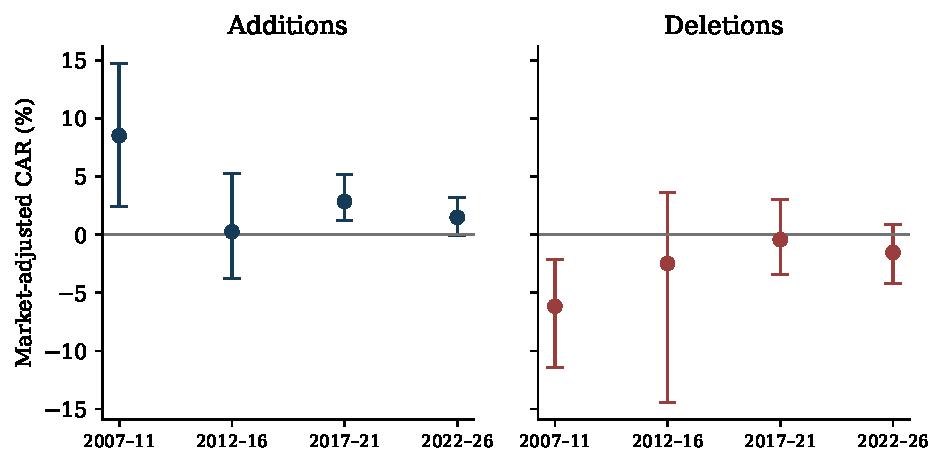
\includegraphics[width=.96\linewidth]{figures/period_returns.pdf}
\caption{Returns around OMXSB changes by period. Points are event-weighted mean CARs from AD-1 through ED+1; bars are the 95\% review-cluster wild-bootstrap intervals reported in Table~\ref{tab:returns}. The vertical scale is identical for additions and deletions. Periods begin in July 2007 and end in June 2026. The estimates describe observed index events, not a fitted trend.}\label{fig:period_returns}
\end{figure}

Deletions have negative means in all four periods: -6.16\%, -2.47\%, -0.43\% and -1.53\%. Their intervals are generally wider than those for additions. In particular, the 2012--2016 deletion estimate is sensitive to the weighting of large reviews. The sign of the averages is consistent with the conventional index-event pattern, but the sample does not precisely resolve the magnitude of recent deletion returns.

The published US finding in \citet{greenwood2025} is a useful benchmark for the question, not a directly comparable control group. Their published abstract reports an average S\&P 500 addition return below 1\% and deletion return of 0.1\% in 2010--2020. Sweden's later interval begins in 2017 and ends in 2026, uses a different benchmark and review institution, and contains different firms. We consequently ask whether a similarly small return is evident within the Swedish series, rather than subtracting the US number and calling the difference a country effect.

For 2017--2026 as a whole, addition CAR averages 2.15\%, with a 95\% interval of [1.01\%, 3.39\%], across 169 events and 19 reviews. The corresponding deletion mean is -1.04\%, with an interval of [-2.88\%, 0.90\%]. These are economically different levels of precision. 

The latest addition estimate, 1.50\%, has an interval of [-0.10\%, 3.22\%]. This permits both a near-zero average and a positive return of economically meaningful size. It does not establish disappearance. The latest block contains only nine review clusters, and its mean is sensitive to particular observations and overlapping index events, as shown below.

The direct time contrasts sharpen the answer. Latest minus earliest addition CAR is -7.03 percentage points, whereas latest minus preceding is -1.35 points, later minus earlier decade is -1.24 points, and the annual linear trend is -0.28 points. Only the endpoint contrast has a pointwise bootstrap interval excluding zero; that result does not survive the limited ten-test multiplicity adjustment. Table~\ref{tab:contrasts} in the appendix reports all contrasts. The evidence is therefore strongest for a high earliest-period mean and a positive later-decade association, rather than a statistically established smooth decline.

\subsection{The changing announcement calendar}

The full-window comparison covers the entire interval between announcement and implementation. In Sweden, that interval changes substantially. Among reviews represented in the complete addition sample, its median is 14, 16, 15 and 6 trading days in the four blocks. Thus, the latest full window is considerably shorter than the typical earlier window. This is a feature of the institution and measurement, not evidence by itself that timing caused any return difference.

We therefore calculate a fixed initial seven-day window, AD-1 through AD+5, on the same events as the full-window means. It contains seven daily returns and ends before implementation for every event. This choice was made after inspecting the event calendar, and the exercise is exploratory. Table~\ref{tab:timing} reports both windows and the remaining portion of the full window.

\begin{table}[!htbp]
\centering
\caption{The full event window and a common initial seven-day window}\label{tab:timing}
\small
\setlength{\tabcolsep}{5pt}
\begin{tabular}{llrrrrr}
\toprule
Type & Period & Events & Gap & Full & Initial seven & Remainder \\
\midrule
Addition & 2007--2011 & 33 & 14 & 8.52 & 1.19 & 7.34 \\
Addition & 2012--2016 & 54 & 16 & 0.25 & 1.26 & -1.01 \\
Addition & 2017--2021 & 82 & 15 & 2.85 & 1.23 & 1.62 \\
Addition & 2022--2026 & 87 & 6 & 1.50 & 1.80 & -0.31 \\
Deletion & 2007--2011 & 33 & 15 & -6.16 & -3.54 & -2.62 \\
Deletion & 2012--2016 & 46 & 16 & -2.47 & -0.86 & -1.61 \\
Deletion & 2017--2021 & 61 & 15 & -0.43 & -1.82 & 1.39 \\
Deletion & 2022--2026 & 75 & 6 & -1.53 & -0.76 & -0.77 \\
\bottomrule
\end{tabular}
\begin{minipage}{\linewidth}\footnotesize\vspace{5pt}
Returns are percentages. Gap is the median AD-to-ED distance in trading days across distinct reviews represented in the sample. Full includes AD-1 through ED+1; Initial seven includes AD-1 through AD+5; Remainder includes AD+6 through ED+1. Every row uses identical events and the two components sum to Full. The remainder has varying duration. This timing diagnostic is exploratory; uncertainty for period contrasts is reported in Appendix~\ref{app:inference}.
\end{minipage}
\end{table}


The addition initial seven-day means are 1.19\%, 1.26\%, 1.23\% and 1.80\%. The very high 8.52\% earliest full-window mean is therefore not a comparably high initial seven-day response: approximately 7.34 percentage points accrue in the remaining interval. In the latest block, the remainder is approximately -0.31 points. These are within-sample accounting comparisons; they do not establish that the initial seven-day population means are equal or that shortening the calendar explains the difference causally.

The distinction matters for the replication's economic interpretation. A declining full-event CAR need not be a declining immediate response to the announcement. It may reflect where returns occur along an episode whose duration also changes. Both parts of the evidence should be visible. The full window remains appropriate for the entire index change, while the fixed window prevents the early large CAR from being described as a large announcement-week reaction without checking its timing.

Return aggregation is a separate issue. On the same 169 later additions, replacing the arithmetic daily sum with compounded stock return minus compounded benchmark return changes the mean from 2.15\% to 2.18\%. In the latest block it changes 1.50\% to 1.45\%. The positive pooled later association is not created by this particular aggregation choice. Alternative closing-price endpoints are also shown in Appendix~\ref{app:data}; the daily return inclusion convention is kept explicit rather than treated as interchangeable with the window label.

\subsection{Firm characteristics and prior returns}

Following the anchor study, we next ask whether changing observable characteristics account for the time pattern. Table~\ref{tab:composition} compares unadjusted and adjusted period estimates on identical complete-case samples. For latest-period additions, the estimate is 1.59\% without controls and 1.60\% with them. For early additions, the corresponding values are 8.97\% and 10.12\%. These controls do not explain away the difference in this specification.

\begin{table}[!htbp]
\centering
\caption{Composition adjustment on a common event sample}\label{tab:composition}
\small
\setlength{\tabcolsep}{5pt}
\begin{tabular}{llrrl}
\toprule
Type & Period & Unadjusted & Adjusted & Adjusted CR1 interval \\
\midrule
Addition & 2007--11 & 8.97 & 10.12 & [5.09, 15.16] \\
Addition & 2012--16 & 0.74 & 0.55 & [-3.01, 4.11] \\
Addition & 2017--21 & 2.64 & 2.33 & [0.38, 4.29] \\
Addition & 2022--26 & 1.59 & 1.60 & [0.68, 2.53] \\
Deletion & 2007--11 & -5.66 & -6.23 & [-11.03, -1.43] \\
Deletion & 2012--16 & -1.37 & -1.42 & [-7.61, 4.76] \\
Deletion & 2017--21 & -0.77 & -0.29 & [-3.35, 2.77] \\
Deletion & 2022--26 & -1.83 & -1.95 & [-4.02, 0.12] \\
\bottomrule
\end{tabular}
\begin{minipage}{\linewidth}\footnotesize\vspace{5pt}
Period intercepts from CAR $[AD-1,ED+1]$ regressions. Both columns use the same complete-case sample: 237 additions or 185 deletions. Adjusted estimates control for centered abnormal turnover, relative size, residual return variance and analyst coverage. The columns are not a causal decomposition. Intervals are analytical CR1 review-clustered intervals using $t_{G-1}$; unstable inverted bootstrap intervals from auxiliary sparse specifications are not used here. Source: Authors' calculations; exact inputs are listed in the replication package.
\end{minipage}
\end{table}


The comparison is conditional on the available turnover, size, residual-variance and analyst-coverage proxies. It does not prove that composition is irrelevant. Missing controls reduce the sample to 237 additions and 185 deletions, and the proxies do not capture all reasons for membership changes. The common-sample unadjusted column is important: comparing an adjusted result with a larger raw sample would otherwise attribute selection from missing controls to the controls themselves.

Coincident MSCI changes matter for magnitudes. Excluding them lowers the later addition mean from 2.15\% to 1.46\%, with an interval of [0.50\%, 2.47\%]. The latest mean falls from 1.50\% to 0.73\%, with an interval including zero. Overlapping events have unusually large returns. This is a Swedish counterpart to asking whether index-specific institutional details change measured demand, but it is not the US migration mechanism: removing an overlap does not identify the incremental causal contribution of either index.

Table~\ref{tab:robustness} also excludes Sivers separately, applies winsorization, and removes observations flagged in a targeted company-news review. The later-decade addition mean remains positive with an interval excluding zero in these individual checks. The latest-block mean is more sensitive. The news screen covers the 24 most extreme events, so its remaining observations cannot be described as comprehensively news-free.

\begin{table}[!htbp]
\centering
\caption{Sensitivity of addition returns}\label{tab:robustness}
\small
\setlength{\tabcolsep}{5pt}
\begin{tabular}{llrrl}
\toprule
Period & Specification & $N$ & CAR & 95\% interval \\
\midrule
2017--26 & Baseline & 169 & 2.15 & [1.01, 3.39] \\
2017--26 & Without MSCI overlap & 157 & 1.46 & [0.50, 2.47] \\
2017--26 & Without screened company news & 163 & 1.91 & [1.01, 2.82] \\
2017--26 & Winsorized 1st and 99th percentiles & 169 & 1.92 & [0.91, 3.05] \\
2017--26 & Without Sivers & 168 & 1.71 & [0.57, 2.96] \\
2022--26 & Baseline & 87 & 1.50 & [-0.10, 3.22] \\
2022--26 & Without MSCI overlap & 82 & 0.73 & [-0.77, 2.32] \\
2022--26 & Without screened company news & 84 & 1.30 & [0.12, 2.43] \\
2022--26 & Winsorized 1st and 99th percentiles & 87 & 1.04 & [-0.11, 2.25] \\
2022--26 & Without Sivers & 86 & 0.62 & [-0.85, 2.23] \\
\bottomrule
\end{tabular}
\begin{minipage}{\linewidth}\footnotesize\vspace{5pt}
Event-weighted CAR $[AD-1,ED+1]$ in percent, with pointwise restricted wild cluster bootstrap intervals by review. Each exclusion is applied separately. The company-news screen examines the 24 most extreme events, rather than the full event universe, and is outcome-informed. MSCI exclusion changes the target population. Winsorization changes the outcome. These are sensitivity descriptions, not independent replications or specification selection rules. Source: Authors' calculations; exact inputs are listed in the replication package.
\end{minipage}
\end{table}


Anticipation is another explanation considered by Greenwood and Sammon. The Swedish additions have positive pre-announcement performance over a long horizon: CAR from AD-100 through AD-1 averages 12.11\%, 18.05\%, 11.82\% and 18.88\% across the four periods. Over the shorter AD-20 through AD-1 window, the means are 0.32\%, 4.11\%, 0.60\% and 2.94\%. Neither sequence shows a steady rise that mirrors the full-window decline.

\begin{table}[!htbp]
\centering
\caption{Pre-announcement returns}\label{tab:anticipation}
\small
\setlength{\tabcolsep}{5pt}
\begin{tabular}{llrrrr}
\toprule
Type & Period & $N_{20}$ & AD-20 to AD-1 & $N_{100}$ & AD-100 to AD-1 \\
\midrule
Addition & 2007--11 & 36 & 0.32 & 31 & 12.11 \\
Addition & 2012--16 & 54 & 4.11 & 51 & 18.05 \\
Addition & 2017--21 & 83 & 0.60 & 80 & 11.82 \\
Addition & 2022--26 & 84 & 2.94 & 81 & 18.88 \\
Deletion & 2007--11 & 32 & -5.56 & 31 & -16.40 \\
Deletion & 2012--16 & 46 & -3.70 & 43 & -9.31 \\
Deletion & 2017--21 & 62 & 0.54 & 62 & -10.26 \\
Deletion & 2022--26 & 74 & -0.48 & 70 & -21.80 \\
\bottomrule
\end{tabular}
\begin{minipage}{\linewidth}\footnotesize\vspace{5pt}
Arithmetic market-adjusted returns in percent. Each window uses its own complete cases and includes AD-1, which also belongs to the primary event window. The columns cannot be added to the main-window mean. Positive prior performance is consistent with anticipation but also with selection on earlier returns; it does not distinguish these channels.
\end{minipage}
\end{table}


These pre-announcement returns may reflect anticipation, but selection on earlier price and trading performance can also generate them. The historical Nasdaq eligibility rule is not reconstructed sufficiently to separate the two. The pre-announcement windows also use their own complete cases and include AD-1; they cannot simply be added to the full-window mean. Appendix~\ref{app:replication} reports the longer AD-20-to-ED+1 demand-ratio counterpart used in the original study.

Taken together, composition adjustment, overlap exclusions and pre-announcement returns narrow the explanations without selecting one. Observed characteristics do not remove the pattern in the matched sample; overlapping events have higher sample returns, but the mean remains positive when they are excluded; and earlier returns do not establish a progressively stronger anticipation mechanism. These are useful findings even though they do not constitute causal decompositions.

\subsection{Reported fund purchases}

The next step follows Greenwood and Sammon's link between the amount bought by trackers and the associated price response. Table~\ref{tab:demand_main} reports the mean sign-adjusted CAR, measured purchases or sales, and their ratio on exactly the same events. Every figure has a straightforward economic unit: demand is a percentage of shares outstanding, and $M$ is percentage points of return per percentage point of measured ownership change.

\begin{table}[!htbp]
\centering
\caption{Observed fund trading and return per unit of measured demand}\label{tab:demand_main}
\small
\setlength{\tabcolsep}{5pt}
\begin{tabular}{llrrrrl}
\toprule
Type & Period & Events & Return & Demand & $M$ & 95\% ratio set \\
\midrule
Addition & 2007--11 & 8 & 8.78 & 0.15 & 57.87 & [-9.55, 471.88] \\
Addition & 2012--16 & 27 & -1.94 & 0.52 & -3.76 & [-15.09, 4.24] \\
Addition & 2017--21 & 58 & 3.29 & 1.11 & 2.97 & [-0.14, 6.30] \\
Addition & 2022--26 & 78 & 2.28 & 0.97 & 2.35 & [-0.21, 4.73] \\
Addition & 2017--26 & 136 & 2.71 & 1.03 & 2.63 & [0.91, 4.37] \\
Deletion & 2007--11 & 7 & -0.19 & 0.26 & -0.72 & All real values \\
Deletion & 2012--16 & 25 & 2.07 & 0.48 & 4.36 & [-17.73, 30.17] \\
Deletion & 2017--21 & 40 & 0.20 & 0.99 & 0.20 & [-4.05, 4.89] \\
Deletion & 2022--26 & 68 & 1.66 & 1.18 & 1.41 & [-0.87, 2.83] \\
Deletion & 2017--26 & 108 & 1.12 & 1.11 & 1.01 & [-0.88, 2.61] \\
\bottomrule
\end{tabular}
\begin{minipage}{\linewidth}\footnotesize\vspace{5pt}
Return is sign-adjusted CAR from AD-1 through ED+1, in percent. Demand is the sign-adjusted broad benchmark-linked holdings change as a percentage of shares outstanding. For deletions, negative returns and sales have positive signs. Each ratio divides the two means on identical events retained after the share-adjustment screen. Joint ratio uncertainty is described in Appendix~\ref{app:inference}; it can be unbounded when the denominator is weak. These are descriptive ratios, not identified elasticities.
\end{minipage}
\end{table}


For additions in 2017--2026, the common holdings sample contains 136 events. Mean CAR is 2.71\%, mean measured demand is 1.03\% of shares outstanding, and their ratio is 2.63. The return exceeds the all-event mean of 2.15\% because the samples differ. The ratio does not imply that an exogenous purchase of 1\% causes a 2.63\% price rise; it describes the relation between two sample averages under the observed fund coverage.

The ratio of means is distinct from the relation across individual events. In a simple regression of signed returns on measured demand with an intercept, purchases explain approximately 0.28\% of return variation across all 171 complete addition observations and 2.49\% across 140 deletions. These descriptive fits retain the complete holdings sample and do not control for other return determinants. They show why the ratio cannot be read as evidence that the stocks bought most by the covered funds necessarily rise most. Measurement error and correlated information also prevent a small fit from ruling out a causal role for demand.

The early addition ratio, 57.87, is especially fragile. It uses only eight events across five reviews, with measured purchases averaging 0.15\% of shares outstanding. Jointly allowing the numerator and denominator to be uncertain gives a 95\% ratio set from -9.55 to 471.88. This large number cannot support a precise claim that Swedish market elasticity has changed by a corresponding factor. The broad later-decade ratio is better resolved, with a set of [0.91, 4.37], while both later five-year ratio sets include zero.

The demand series also needs a coverage interpretation. The broad addition measure is 0.15\%, 0.52\%, 1.11\% and 0.97\% across the four blocks. It rises relative to the sparse early observations but does not increase continuously. Reporting coverage and fund mandates evolve, and the share-adjustment screen removes a much larger proportion of early candidates. The observed historical increase therefore combines investor activity with changes in what can be measured.

\begin{figure}[!htbp]\centering
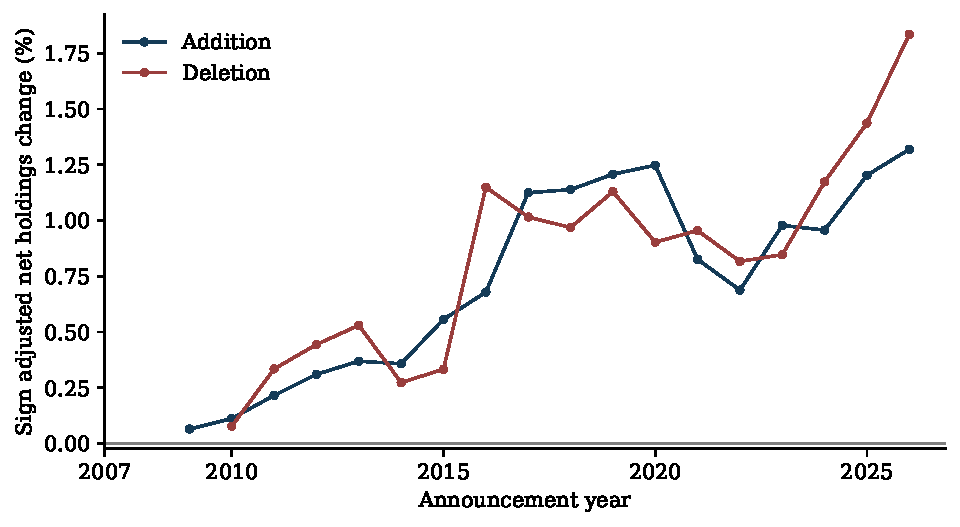
\includegraphics[width=.92\linewidth]{figures/fund_demand.pdf}
\caption{Observed benchmark-linked ownership changes. Annual event means of sign-adjusted net holdings changes as a percentage of shares outstanding. Positive deletion values denote sales. The broad fund definition includes benchmark variants and benchmark-linked mixed-fund holdings. Coverage changes over time; the series is not an estimate of total passive assets or implementation-day orders. The last year is incomplete.}\label{fig:demand}
\end{figure}

The separate FI reporting channel is informative on a matched recent sample. For 106 additions in 2019--2026, measured demand is 1.14\% using FI and 1.05\% using the matched Lipper-based measure. Both use the same mean CAR, 2.43\%, giving ratios of 2.12 and 2.30. This agreement supports the scale of measured later purchases on the overlap. It does not fill missing early reports or establish that either channel captures every relevant investor.

A fixed fund-universe check further separates some coverage change from changes in event composition. Only three funds satisfy the selected mandate and report-availability requirements at every later-decade review; none do so across the whole 2007--2026 period. Within each block, using the same events for the fixed and broad fund measures, fixed-universe addition demand falls from approximately 0.49\% to 0.38\% between the two later blocks, compared with 1.11\% to 0.97\% in the broad measure. The smaller denominator describes a narrower investor population, not a correction that recovers total demand. Appendix~\ref{app:holdings} gives the definition and results.

Purchases are not confined to the benchmark-linked group. Table~\ref{tab:observed_funds} partitions reported fund trading on the same later addition events. Other funds classified as passive buy a further 0.40\% of shares outstanding. Active funds sell approximately 0.24\%, with an interval spanning zero, leaving observed funds collectively as net buyers of 1.19\%. The categories sum within each event; their intervals need not add because their trades covary. These observations do not identify the counterparties or rule out offsetting trades by investors missing from the extract.

\begin{table}[!htbp]
\centering
\caption{Reported fund trading around later additions}\label{tab:observed_funds}
\small
\setlength{\tabcolsep}{5pt}
\begin{tabular}{p{8.2cm}rl}
\toprule
Investor group & Mean purchase & 95\% interval \\
\midrule
Covered OMXSB-linked funds (C) & 1.03 & [0.85, 1.21] \\
Other funds classified as passive & 0.40 & [0.25, 0.55] \\
Funds classified as active & -0.24 & [-0.52, 0.04] \\
All included funds & 1.19 & [0.75, 1.62] \\
\bottomrule
\end{tabular}
\begin{minipage}{\linewidth}\footnotesize\vspace{5pt}
Net purchases as a percentage of shares outstanding on identical 136 additions in 19 reviews, 2017--2026. The first three rows partition included holdings; the final row is their within-event sum. Mixed-fund security holdings are included at their reported amounts, without the benchmark weights used in the separate AUM measure. Intervals use analytical CR1 by review and $t_{G-1}$. These are covered fund positions, not the complete investor population or observed implementation-day orders.
\end{minipage}
\end{table}


The holdings evidence thus supports a measured trading association and a useful recent cross-source comparison. It does not establish a precise long-run elasticity trend. The difference from the anchor's US argument is substantive: here, the historical denominator is too coverage-sensitive to carry a strong claim about how efficiently the market absorbs a fixed amount of demand.

\subsection{Trading at implementation}

The return results do not mean that portfolio adjustment has become unimportant. The final trading day before effectiveness accounts for 9.44\% of the 45-day volume window for early additions and 15.24\% for latest-period additions. The increase is 5.79 percentage points, with a 95\% interval of [3.30, 8.84]. Deletions show a similar increase, from 8.75\% to 14.52\%, a difference of 5.76 points with an interval of [3.26, 8.38].

\begin{figure}[!htbp]\centering
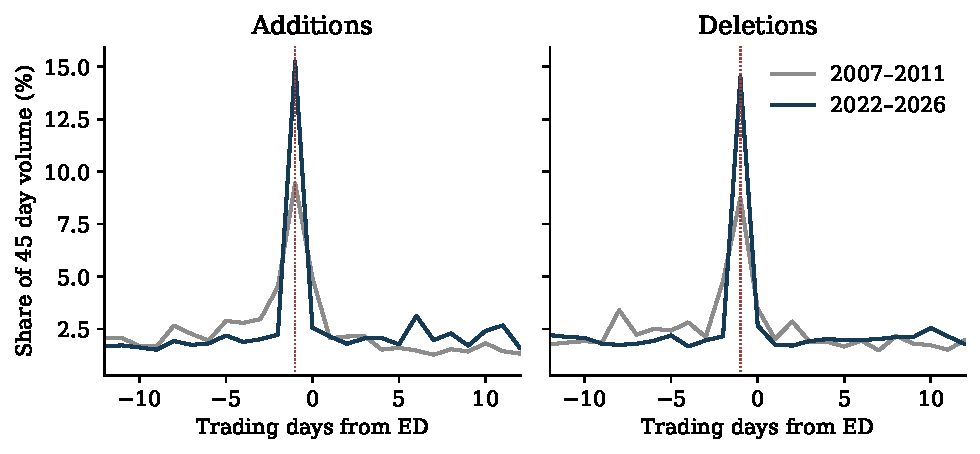
\includegraphics[width=.96\linewidth]{figures/volume_concentration.pdf}
\caption{Trading concentrates immediately before effectiveness. Daily volume as a percentage of each event's total over ED-22 through ED+22; the graph displays ED-12 through ED+12. The dotted line marks ED-1, the final trading day before the new portfolio takes effect. Missing volume is set to zero in this measure. Daily observations do not separate auction and continuous trading.}\label{fig:volume}
\end{figure}

More concentrated trading can coexist with a small implementation-window return. The latest addition implementation CAR is -0.09\%, whereas the announcement CAR is 1.20\%. Investors may anticipate demand or supply liquidity when funds rebalance; prices may also respond to information at other points in the interval. The daily data do not identify which explanation dominates. What they do establish is that the distribution of measured trading around implementation changes even when the mean return near implementation is small.

The spread series supplies context. The value-weighted closing quoted spread among OMXSB members falls from 0.270\% in 2007 to 0.079\% in 2025; the partial 2026 value is 0.087\%. This is consistent with lower quoted trading frictions. It is a different object from the effective spreads and implementation costs examined in the US paper. A closing quote does not measure market depth or the price impact of a large predictable order, so the spread decline cannot establish that improved liquidity caused the return pattern. The annual series is retained in Appendix~\ref{app:additional}.



\subsection{Returns after implementation}

Temporary trading pressure is one possible explanation for index-event returns. To describe their subsequent path, we extend the horizon through ED+20 and retain exactly the same events for every plotted day. The return before implementation runs from AD-1 through ED-1; the after-implementation component runs from ED through ED+20. Their sum includes every day once. This is a separate exploratory extension: Greenwood and Sammon's longer demand-ratio window instead starts earlier, at AD-20, and ends at ED+1.

\begin{figure}[!htbp]\centering
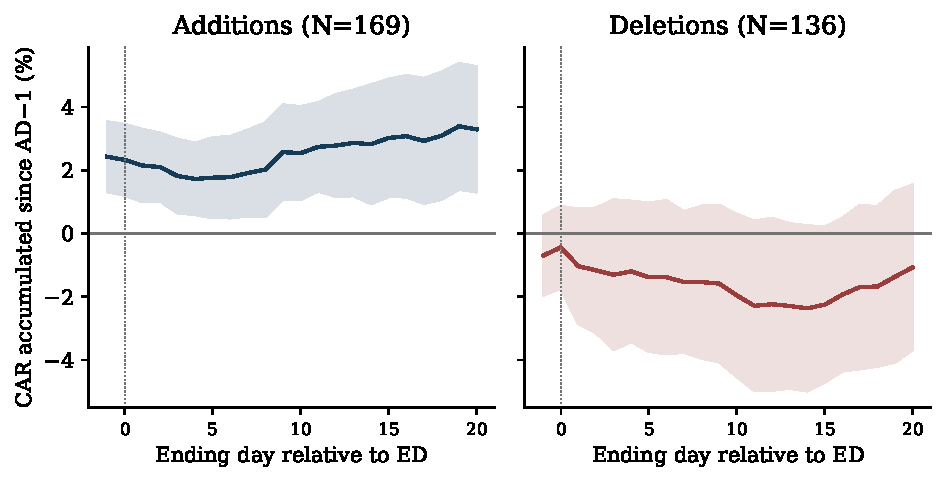
\includegraphics[width=.96\linewidth]{figures/fixed_cohort_path.pdf}
\caption{Cumulative performance through twenty days after implementation. The cohort is fixed separately for additions and deletions in 2017--2026. At every point, the cumulative return starts at AD-1; the horizontal axis gives its ending day relative to ED. The first plotted point is therefore the return already accumulated through ED-1, not a zero normalization. Shading gives pointwise 95\% analytical intervals clustered by review, not a simultaneous confidence band. Counts are 169 additions and 136 deletions.}\label{fig:path}
\end{figure}

\begin{table}[!htbp]
\centering
\caption{Returns before and after implementation on a fixed cohort}\label{tab:horizon_main}
\small
\setlength{\tabcolsep}{5pt}
\begin{tabular}{llrrrrl}
\toprule
Type & Period & Events & Before & After & Cumulative & 95\% interval \\
\midrule
Addition & 2017--2026 & 169 & 2.43 & 0.87 & 3.30 & [1.31, 5.28] \\
Addition & 2022--2026 & 87 & 1.77 & -0.06 & 1.71 & [0.72, 2.69] \\
Deletion & 2017--2026 & 136 & -0.70 & -0.38 & -1.07 & [-3.68, 1.54] \\
Deletion & 2022--2026 & 75 & -0.93 & -0.95 & -1.88 & [-5.72, 1.96] \\
\bottomrule
\end{tabular}
\begin{minipage}{\linewidth}\footnotesize\vspace{5pt}
Returns in percent. Before is AD-1 through ED-1; After is ED through ED+20; Cumulative is AD-1 through ED+20. Each row uses the same events throughout. Intervals are analytical CR1 with review clustering for the cumulative mean. Separate wild-bootstrap tests and post-result exclusions are in the appendix. The horizon is finite and the analysis exploratory.
\end{minipage}
\end{table}


For later-decade additions, the pre-implementation mean is 2.43\% and the subsequent component is 0.87\%, giving 3.30\% cumulatively. The cumulative analytical interval is [1.31\%, 5.28\%]. The after-implementation component's interval is [-0.78\%, 2.51\%], so the result does not establish a separately positive drift after the index change. It shows that the measured cumulative average has not returned to zero by the selected horizon.

The latest block illustrates why a longer horizon must not be selected simply because it produces a smaller $p$-value. Its cumulative estimate is 1.71\%, with an interval of [0.72\%, 2.69\%], but falls to 1.25\% without Sivers and 1.21\% without MSCI overlaps; both latter intervals include zero. The pooled later-decade cumulative mean remains positive in those separate checks. The exclusions were examined after the extension's results were observed. All are reported as exploratory sensitivities, not independent confirmations.

Deletion cumulative returns are less precisely resolved: -1.07\% in 2017--2026 and -1.88\% in the latest block, with both intervals spanning zero. Neither side of the exercise establishes permanent price impact. Twenty trading days remain a finite horizon, and selection, subsequent news and benchmark error can affect cumulative performance throughout it.

\subsection{Comparison securities and share classes}

A separate size-screened comparison provides a complementary check. After removing the one-day overlap between its pre-return control and outcome, the later addition coefficient is 1.65 percentage points, with a 95\% analytical interval of [0.48, 2.83]. Restricting comparisons to the main market gives 1.49 points, with an interval of [0.24, 2.74]. The correction preserves the sample and other controls. These remain conditional differences rather than threshold-based causal estimates; Appendix~\ref{app:comparisons} reports the full before-and-after results.

Swedish firms with multiple listed share classes offer an additional comparison. Both classes are exposed to much of the same firm information, while only one may be involved in the index event. If class-specific demand is important, their relative performance is informative. This design improves on a comparison with an unrelated firm in one respect, but it does not make the other class untreated: substitution, arbitrage and shared investor attention can transmit the event to it.

\begin{table}[!htbp]
\centering
\caption{The indexed and sister share classes on the same events}\label{tab:twins}
\small
\setlength{\tabcolsep}{5pt}
\begin{tabular}{lrrrrr}
\toprule
Events & Count & Firms & Index class & Sister class & Difference \\
\midrule
Addition & 19 & 10 & 2.13 & 2.48 & -0.34 \\
Deletion & 20 & 11 & 4.17 & 3.20 & 0.97 \\
Combined & 39 & 13 & 3.18 & 2.85 & 0.33 \\
\bottomrule
\end{tabular}
\begin{minipage}{\linewidth}\footnotesize\vspace{5pt}
Sign-adjusted log market-excess returns in percent for AD-1 through ED+1. Deletion signs are reversed. Each difference subtracts the sister-class mean from the index-class mean on identical events. The combined sample contains 39 events from 13 distinct firms; firm counts by event type overlap. The combined relative-return placebo $p$-value is 0.407. These selected log-return observations cannot be subtracted from the main arithmetic-CAR sample to identify a causal component.
\end{minipage}
\end{table}


Table~\ref{tab:twins} reports both return legs on identical events. Across 39 events from 13 firms, the index-class mean is 3.18\% and the sister-class mean 2.85\%, leaving a relative return of 0.33 percentage points (placebo $p=0.407$). These selected observations use sign-adjusted log market-excess returns. They cannot be subtracted from the 2.15\% main arithmetic-CAR estimate as a causal decomposition.

The small relative estimate does not establish that index demand has no effect. Some of the difference may be transmitted to the sister class; some firms occur repeatedly; and thin trading or changes in return sources affect the measurement. A source-consistent subset contains 29 events from nine firms and has a relative mean near 0.04 points. The placebo construction does not jointly preserve all firm and review dependence. This extension therefore indicates that the available within-firm sample does not precisely isolate a class-specific response, while keeping both stock legs visible rather than treating the comparison as an unexplained null.




\FloatBarrier

\section{Discussion}\label{sec:discussion}
\subsection{What remains of the index effect}

The replication answers the return question more clearly than the mechanism question. Additions retain a positive average market-adjusted return over 2017--2026, including when influential returns and coincident index events are excluded separately. The later return also exceeds that of the size-screened comparison securities after correcting the overlapping control window. The latest five-year estimate is less precise and more sensitive to individual events. The defensible answer is that a positive addition association remains in the later decade, while its current magnitude is not precisely established. Deletions provide weaker evidence because their intervals permit materially different return magnitudes.

This result is relevant to \citet{greenwood2025} because the disappearance they document is an empirical development, not an automatic consequence of the growth of indexing. Sweden supplies another setting in which to examine the same questions. Reported benchmark-linked purchases and implementation trading are clearly visible, yet the pooled later addition return remains positive. This extends the institutional scope of the question without establishing that otherwise identical Swedish and US stocks respond differently. The periods, selection procedures, investor populations and measurement conventions differ.

The comparison must also distinguish the anchor's pooled S\&P 500 result from its migration analysis. When an addition to one tracked index is a deletion from another, purchases by the destination's trackers need not measure net index-related demand. We have not reconstructed an equivalent historical system of Swedish origin and destination indices. Purchases by other passive funds and the large returns of coincident MSCI events are informative about our sample, but do not prove that offsetting demand is absent elsewhere. The Swedish contribution consequently does not depend on treating every addition as a verified direct addition.

\subsection{What the trading evidence explains}

Fund holdings make the return result economically more informative. On the same later addition events, covered benchmark-linked funds purchase 1.03\% of shares outstanding and CAR averages 2.71\%. Their ratio of 2.63 describes how much return accompanies a percentage point of measured purchases. It is not the slope from an experiment in which demand alone changes. The holdings-report interval also differs from the return window, so the ratio should not be described as an immediate response to orders submitted at implementation.

Two issues prevent that interpretation. First, membership follows firm characteristics and prior performance. News or investor attention can move prices during the window even after market adjustment. Second, observed funds cover only part of the investor population. Omitted institutions can buy or sell, and absent security positions can be inferred as zero. A partial sum of net trades is therefore not necessarily a lower bound on total net index-related demand. Coverage can change the measured ratio even if the response to an otherwise identical order remains unchanged.

The FI comparison strengthens a specific part of the measurement: recent reported purchases have a similar scale through two reporting channels. It does not authenticate every historical zero position or establish constant coverage. The fixed-fund sensitivity also describes a narrower population rather than recovering missing investors. Its mean purchases fall between the two later blocks. Together, these checks support using recent holdings to describe trading, while limiting a claim that rising total passive demand explains a precisely measured historical multiplier decline.

Quoted spreads and daily volume describe the accompanying trading environment. Narrower spreads coexist with more concentrated trading immediately before effectiveness. A small implementation-window return is compatible with investors anticipating the trades or supplying liquidity when they occur. It is also compatible with prices responding earlier to information associated with selection. Closing quotes and daily volume do not distinguish these channels. They show why a small return near implementation need not mean that reconstitution trading has become unimportant.

\subsection{Timing and the nature of the remaining return}

The timing extension changes the description of the historical decline. The first-to-last addition difference is -7.03 percentage points for the full episode and +0.62 points for the common initial seven daily returns. The latter interval, [-1.80, 3.03], establishes neither equality nor an increase. The remaining interval accounts for -7.64 points of the full contrast. The unusually high early total return is principally accumulated after the common initial interval, during episodes that generally allowed more time before implementation. This is a concrete measurement finding even though duration, firm composition and intervening information cannot be separated causally.

The subsequent path addresses a different question. On the fixed later-decade cohort, cumulative CAR is 3.30\% through ED+20. The observed average has not returned to zero by that horizon. This is more informative than treating an insignificant post-event coefficient as proof of no reversal, but it does not identify a permanent index premium. The counterfactual return is unknown, the horizon was examined after the original results, and the latest-block estimate is sensitive to exclusions.

The sister-class comparison asks whether the movement is confined to the security whose status changes. In its selected sample, the index class and sister class have sign-adjusted log market-excess means of 3.18\% and 2.85\%, leaving an imprecise difference of 0.33 points. Shared firm information is one possible explanation. Substitution and arbitrage can also transmit demand between related classes, while voting rights, liquidity and investor clienteles differ. An unchanged index status therefore does not make the sister class unaffected. The small relative estimate neither proves a shared-information explanation nor supplies a causal upper bound on class-specific index demand.

The later-decade path and the separately selected share-class sample describe different aspects of observed returns. Several mechanisms remain compatible with both findings. Documenting returns around changes is a different task from assigning those returns to the orders of particular funds. The former is supported more directly here than the latter.

\subsection{Scope and implications}

Historical notice fields and corporate actions are not fully reconciled. Return availability and the holdings adjustment screen select changing samples, particularly early in the history. Moreover, many securities do not create many independent reviews: the latest block contains nine review clusters, and the research includes several retrospective specifications. The appendix records unresolved source issues and retains unfavorable as well as favorable sensitivities. These limitations are especially consequential for the historical multiplier, less directly for the independently reproduced later return mean.

The estimates are not a tested investment strategy. They neither deduct trading costs nor demonstrate that additions were predictable before the public notice. For research on indexing, the useful finding is that a later addition association coexists with reported benchmark buying and more concentrated trading, while its attribution remains unresolved. The combination of return and holdings evidence extends the anchor question without requiring a structural demand estimate.

A sharper mechanism test would require evidence that separates the competing accounts. Complete historical portfolios would help reconcile omitted positions and changing fund coverage. Class-specific transactions and investor identities would help distinguish direct purchases from substitution across classes. A credible source of membership or demand variation unrelated to firm news would be needed for causal attribution; more controls alone would not provide it. These requirements follow from the findings. The present study establishes what remains in the observed return series and why its timing and investor coverage matter for interpretation.
\FloatBarrier

\clearpage
\section{Conclusion}

This thesis examines whether the disappearing index effect documented by \citet{greenwood2025} also appears around OMXSB reconstitutions. The Swedish return pattern shows substantial historical attenuation, but no monotonic decline. Additions earn 8.52 \% in 2007--2011 and 1.50 \% in 2022--2026. Across the later decade, the mean is 2.15 \%, with a 95 \% interval of 1.01 to 3.39 \%. The latest block alone is less precise and sensitive to influential events. These findings support a positive later-decade addition association; they establish neither economic disappearance nor a stable current premium.

Reported fund trading and pre-implementation volume confirm that index changes coincide with concentrated benchmark-related activity. In the common later addition sample, covered purchases average 1.03 \% of outstanding shares. The return-to-purchases ratio is 2.63, but changing coverage, broad reporting intervals and potentially shared information prevent a structural interpretation. Regulatory holdings provide a useful check on the later demand scale.

Two extensions sharpen the interpretation. The earliest-to-latest return decline is concentrated after a common initial seven-return window, while the announcement-to-implementation interval becomes shorter. This is a measurement decomposition, not evidence that calendar changes caused the decline. In the selected share-class sample, both classes move substantially and their relative return is imprecise. That pattern is compatible with shared information or demand transmitted across classes; it does not isolate either mechanism.

The Swedish evidence consequently answers the persistence question more clearly than the mechanism question. Positive average addition returns remain in the later sample, alongside observable fund buying, but the data do not identify the causal contribution of that buying. More complete investor coverage, reconciled holdings histories and transaction-level evidence would help distinguish changes in demand from changes in the market's ability to accommodate it.

\FloatBarrier
\clearpage
\bibliographystyle{apalike}
\bibliography{references}
\clearpage
\appendix
\setcounter{table}{0}
\renewcommand{\thetable}{A\arabic{table}}
\setcounter{figure}{0}
\renewcommand{\thefigure}{A\arabic{figure}}
\section{Replication details and source versions}
\label{app:replication}

This study replicates and extends the empirical framework of \citet{greenwood2025} in Sweden. The detailed comparison uses their March 2024 author manuscript, deposited in Harvard DASH under the 2025 publication record \citep{greenwood2024ms}. That manuscript is not authenticated as the final published text: its abstract reports a recent deletion return of 0.1\%, while its body retains an older estimate of $-0.6$\%. Published headline comparisons therefore use the journal's abstract; the method references below identify the March 2024 version explicitly. The published full text and official replication files were not accessible for this review, leaving program-level equivalence unresolved.

The author manuscript's Equation~(2) defines excess cumulative stock returns relative to the S\&P~500 over announcement, implementation and announcement-to-implementation windows. Its Equation~(1) motivates a price multiplier $M$ applied to measured demand $D$. The Swedish analysis preserves these organizing questions, replacing the benchmark with OMXSBGI. It adapts the event screens, investor classifications, reporting intervals and inference to the available Swedish data. In particular, review clustering differs from the White standard errors in the original main tables; many Swedish securities change membership simultaneously.

\begin{table}[H]
\centering
\caption{From Greenwood--Sammon to the Swedish implementation}\label{tab:replication_map}
\small
\setlength{\tabcolsep}{5pt}
\begin{tabular}{p{2.0cm}p{4.65cm}p{6.1cm}}
\toprule
Component & Anchor study & Swedish analysis \\
\midrule
Return pattern & S\&P 500 additions/deletions; announcement, implementation and full windows & OMXSB; same event-window questions, explicitly defined daily-sum CAR \\
Time comparison & Long US history and decade means & Four Swedish calendar blocks and two pooled decades; incomplete 2026 \\
Composition & Period indicators and four firm characteristics & Same regression structure; Swedish measurement proxies and common samples \\
Index demand & Tracking-trade classification; quarterly holdings & Dated mandate groups; available pre/post reports; FI comparison \\
Other index activity & Migrations within S\&P index families & Coincident MSCI changes; a distinct overlap diagnostic \\
Anticipation & Pre-announcement returns and longer starting window & Pre-return windows and AD-20 to ED+1 ratio; historical eligibility not fully reconstructed \\
Liquidity & Effective spreads and implementation costs & Closing quoted spreads and daily volume concentration \\
Extensions & Anchor comparison provides the baseline & Fixed-duration timing, within-firm share classes and separate holdings reporting \\
\bottomrule
\end{tabular}
\begin{minipage}{\linewidth}\footnotesize\vspace{5pt}
The mapping distinguishes conceptual replication from exact numerical reproduction. Detailed source-version references and adaptations appear in Appendix~\ref{app:replication}. Differences in periods, sample selection, holdings dates and return conventions prevent interpreting raw cross-country differences as causal effects.
\end{minipage}
\end{table}


The US tracker classification uses the average annual share of index trades and a 50\% threshold. Swedish production estimates instead use curated, dated fund classifications. The US observations straddle quarterly reports, while Swedish snapshots are sought before AD and after ED. The original acquisition and listing screens also differ from the Swedish offer/delisting exclusions. These departures preclude describing the exercise as an exact reproduction. Likewise, MSCI overlap is a concurrent-event sensitivity, not a reconstruction of the original S\&P index-family migration mechanism.

The four composition controls retain the original categories: abnormal turnover, relative size, residual variance and analyst coverage. Their construction is adapted: the Swedish monthly forecast count need not equal the original unique-analyst count at the latest earnings announcement. Demand also uses ED shares outstanding rather than the original post-event quarterly denominator. The multiplier with controls scales period indicators by period-average demand; it is not an event-level regression of returns on individual fund purchases.

The pre-announcement exercise follows the original paper's anticipation question, but positive prior returns can also reflect selection on performance. The longer demand-ratio window is AD$-20$ through ED$+1$, as in the author manuscript's Tables~5--6. It should be distinguished from the separate Swedish extension through ED$+20$.

\begin{table}[!htbp]
\centering
\caption{The earlier-start demand-ratio window}\label{tab:long_demand}
\small
\setlength{\tabcolsep}{5pt}
\begin{tabular}{llrrrr}
\toprule
Type & Period & Short $N$ & Short $M$ & Long $N$ & Long $M$ \\
\midrule
Addition & 2007--11 & 8 & 57.87 & 8 & 60.83 \\
Addition & 2012--16 & 27 & -3.76 & 27 & -1.82 \\
Addition & 2017--21 & 58 & 2.97 & 58 & 4.24 \\
Addition & 2022--26 & 78 & 2.35 & 75 & 6.66 \\
Deletion & 2007--11 & 7 & -0.72 & 7 & 12.98 \\
Deletion & 2012--16 & 25 & 4.36 & 25 & 8.49 \\
Deletion & 2017--21 & 40 & 0.20 & 40 & -0.57 \\
Deletion & 2022--26 & 68 & 1.41 & 67 & 2.44 \\
\bottomrule
\end{tabular}
\begin{minipage}{\linewidth}\footnotesize\vspace{5pt}
Short is AD-1 to ED+1; Long is AD-20 to ED+1, the earlier-start counterpart in the anchor study. Each ratio uses identical events in its own numerator and denominator, but the short and long samples can differ. These are descriptive point estimates; the table does not claim well-identified early multipliers. The ED+20 analysis is a separate extension.
\end{minipage}
\end{table}

\FloatBarrier

\section{Return conventions and source checks}
\label{app:data}
\label{app:definitions}

\begin{table}[!htbp]
\centering
\caption{Coverage across periods}\label{tab:sample_by_period}
\small
\setlength{\tabcolsep}{5pt}
\begin{tabular}{llrrrr}
\toprule
Type & Period & Source events & Return sample & Holdings sample & Reviews \\
\midrule
Addition & 2007--2011 & 48 & 33 & 8 & 9 \\
Addition & 2012--2016 & 58 & 54 & 27 & 10 \\
Addition & 2017--2021 & 90 & 82 & 58 & 10 \\
Addition & 2022--2026 & 88 & 87 & 78 & 9 \\
Deletion & 2007--2011 & 54 & 33 & 7 & 9 \\
Deletion & 2012--2016 & 53 & 46 & 25 & 10 \\
Deletion & 2017--2021 & 66 & 61 & 40 & 10 \\
Deletion & 2022--2026 & 79 & 75 & 68 & 9 \\
\bottomrule
\end{tabular}
\begin{minipage}{\linewidth}\footnotesize\vspace{5pt}
The source inventory precedes security matching, exclusions and return requirements. Return sample requires complete AD-1 through ED+1 returns after the stated deletion exclusions. Holdings sample additionally requires the broad demand measure and retention under the share-adjustment screen, with a nonmissing matching return. Reviews counts distinct review cycles in the return sample. The figures describe coverage, not random attrition.
\end{minipage}
\end{table}


The observation is a security--review event; an issuer can recur or contribute different share classes. Dates are mapped to the observed trading calendar. Every stated CAR window includes the daily returns at both endpoints. Thus AD$-1$ is the first included daily return, not the closing-price baseline for the subsequent investment. CAR sums daily percentage stock returns less daily OMXSBGI returns. Stock total returns are used where available, with closing-price returns as a fallback. This convention does not automatically preserve dividends in every fallback observation.

The source manuscript calls its inputs cumulative returns but does not settle the daily aggregation or endpoint conventions sufficiently to authenticate an exact match. Table~\ref{tab:return_conventions} therefore compares arithmetic sums with compounded stock returns minus compounded benchmark returns on identical observations and included days. For 2017--2026 additions, the means are 2.15\% and 2.18\%; in 2022--2026 they are 1.50\% and 1.45\%. Interpreting AD$-1$ as a baseline close instead changes the later-decade mean to approximately 2.75\%. That is a change of included returns, not a compounding result.

\begin{table}[!htbp]
\centering
\caption{Return definitions on matched events}\label{tab:return_conventions}
\small
\setlength{\tabcolsep}{5pt}
\begin{tabular}{llrrrr}
\toprule
Type & Period & Events & Daily sum & Compounded & Base at AD-1 \\
\midrule
Addition & 2007--2011 & 33 & 8.52 & 8.60 & 9.27 \\
Addition & 2012--2016 & 54 & 0.25 & 0.38 & 0.42 \\
Addition & 2017--2021 & 82 & 2.85 & 2.96 & 4.20 \\
Addition & 2022--2026 & 87 & 1.50 & 1.45 & 1.38 \\
Addition & 2017--2026 & 169 & 2.15 & 2.18 & 2.75 \\
Deletion & 2007--2011 & 33 & -6.16 & -6.05 & -6.61 \\
Deletion & 2012--2016 & 46 & -2.47 & -2.38 & -2.62 \\
Deletion & 2017--2021 & 61 & -0.43 & -0.53 & -0.37 \\
Deletion & 2022--2026 & 75 & -1.53 & -1.63 & -1.87 \\
Deletion & 2017--2026 & 136 & -1.04 & -1.14 & -1.20 \\
\bottomrule
\end{tabular}
\begin{minipage}{\linewidth}\footnotesize\vspace{5pt}
Daily sum is the primary arithmetic CAR. Compounded is the stock buy-and-hold return minus the benchmark buy-and-hold return using the same included daily returns, AD-1 through ED+1. Base at AD-1 instead starts from the AD-1 close and includes daily returns AD through ED+1. Both latter columns compound stock and benchmark separately. These are sensitivity checks, not proof of the original US code\textquotesingle{}s convention.
\end{minipage}
\end{table}


The announcement-to-effective lag ranges from six to eighteen trading days. It is generally fourteen to eighteen days during 2010--2019 and six to eight days during 2022--2026. Consequently, the total event window changes duration. The common AD$-1$ through AD$+5$ sensitivity ends before ED in every review; its complement begins at AD$+6$. Their sum exactly recovers the total CAR on the same cohort. The first-to-last addition decline is concentrated in this remainder, whose duration and composition also vary. This accounting does not show that shorter notice caused lower returns.

External research recovered accessible notices or original attachments for 35 of 39 reviews, sometimes through republication; three further reviews were visible only in indexed text. The 2008 second-half notice remained unresolved. A December 2008 correction also prints an inconsistent effective year. Document retrieval is not complete field-level reconciliation, and neither a trading-volume peak nor the label ``effective date'' independently authenticates open-versus-close implementation conventions.
\FloatBarrier

\section{Holdings measurement and coverage}
\label{app:holdings}

Group C combines strict followers, benchmark variants and funds with an OMXSB-linked component. It measures covered positions rather than all passive capital. The numerator reconstructs to numerical precision for all 311 complete primary holdings events. Available timestamps satisfy the stated pre-AD and post-ED limits, but this verifies recorded dates rather than the completeness of the underlying reports. Forty fund-event records use a pre-position date different from the latest fund report identified by the availability check.

An absent position is treated as zero when other reporting establishes fund availability. Among addition records, 1,630 of 1,739 contributing fund-event observations have no observed pre-position row. A zero is plausible for a newly included security, but a security-query extract cannot independently distinguish it from an omitted response. Original reports or vendor completeness information are required to resolve that distinction.

The adjustment exclusion compares a market-capitalization/share-count/adjusted-price proxy at ED with its value at the security's final available price date. A missing ratio or a ratio outside $[1/1.4,1.4]$ triggers exclusion. It is therefore a share-adjustment consistency screen, not simply a record of splits during the event window. Later corporate actions can affect early-event eligibility. This safeguard may be needed because adjusted fund shares are divided by historical shares outstanding; removing it without reconciling vendor conventions would not be a justified correction.

\begin{table}[!htbp]
\centering
\caption{Fund definitions on the broad-measure event sample}\label{tab:holdings_coverage}
\small
\setlength{\tabcolsep}{5pt}
\begin{tabular}{llrrrrr}
\toprule
Type & Period & Events & Strict & + variants & Broad & Mixed count \\
\midrule
Addition & 2007--11 & 8 & 0.10 & 0.15 & 0.15 & 0.0 \\
Addition & 2012--16 & 27 & 0.37 & 0.49 & 0.52 & 0.4 \\
Addition & 2017--21 & 58 & 0.92 & 1.02 & 1.11 & 1.0 \\
Addition & 2022--26 & 78 & 0.41 & 0.78 & 0.97 & 8.8 \\
Deletion & 2007--11 & 7 & 0.20 & 0.26 & 0.26 & 0.0 \\
Deletion & 2012--16 & 25 & 0.31 & 0.46 & 0.48 & 0.1 \\
Deletion & 2017--21 & 40 & 0.83 & 0.92 & 0.99 & 1.0 \\
Deletion & 2022--26 & 68 & 0.52 & 0.93 & 1.18 & 9.4 \\
\bottomrule
\end{tabular}
\begin{minipage}{\linewidth}\footnotesize\vspace{5pt}
Demand is percent of shares outstanding, sign-adjusted for deletions. All three demand definitions in a row use the same retained event sample. Strict comprises exact benchmark followers; the next column adds related benchmark variants; Broad also includes the benchmark-linked mixed-fund category. Mixed count is the mean number of reporting mixed funds per event, not their ownership percentage. These data do not measure the complete investor universe.
\end{minipage}
\end{table}


All 468 stored share denominators and adjustment ratios reconstruct. For the 311 retained holdings observations, the denominator exists on ED in the daily panel, although daily availability does not prove that the underlying issuer disclosure is fresh. The screen removes 26 of 37 early addition candidates, compared with nine of 87 in the latest block, contributing to unequal historical coverage.

A fixed-universe sensitivity intersects verified mandate status and reporting availability across every review, without selecting on purchases or returns. No fund survives all 39 reviews. Three survive the 19 later reviews: Swedbank Robur Access Mix, Swedbank Robur Access Sverige and iShares OMX Stockholm Capped UCITS ETF. Within each block, on the same additions as the broad measure, their mean purchases fall from 0.488\% to 0.378\% between the last two blocks, compared with 1.107\% and 0.973\% for broad C. The narrower measure retains the same missing-position assumptions and omits relevant investors. It supports neither continuously increasing purchases nor a corrected estimate of total index demand.
\FloatBarrier

\section{Statistical inference and sensitivity}
\label{app:inference}

For the event-weighted mean $\widehat\mu=N^{-1}\sum_i y_i$, review-clustered CR1 variance is
\begin{equation}
 \widehat V(\widehat\mu)=\frac{G}{G-1}\frac{1}{N^2}
 \sum_{g=1}^G\left[\sum_{i\in g}(y_i-\widehat\mu)\right]^2,
\end{equation}
where $G$ is the number of reviews. The intercept-only regression's remaining degrees-of-freedom correction equals one. Joint covariance of mean signed returns and demand uses the corresponding two-dimensional review scores.

For the ratio $\widehat M=\overline Y/\overline D$, a candidate value $m$ belongs to the Fieller set if
\begin{equation}
 (\overline Y-m\overline D)^2\leq
 t_{G-1,0.975}^{2}
 \left[\widehat V_{YY}-2m\widehat V_{YD}+m^2\widehat V_{DD}\right].
 \label{eq:fieller}
\end{equation}
This accounts for covariance between numerator and denominator \citep{fieller1954}. Sets can be bounded, unbounded or all real values; weak denominator precision must not be concealed by discarding inconvenient outcomes. With few reviews, the approximation does not guarantee exact coverage. The early addition set spans $[-9.55,471.88]$, while the earliest deletion set contains every real value. These estimates cannot establish a precise historical change in structural elasticity.

\begin{table}[!htbp]
\centering
\caption{Returns scaled by observed benchmark linked fund purchases}\label{tab:demand}
\small
\setlength{\tabcolsep}{5pt}
\begin{tabular}{llrrrrrl}
\toprule
Type & Period & $N$ & $G$ & $\bar Y$ & $\bar D_C$ & $\widehat M$ & Fieller set \\
\midrule
Addition & 2007--11 & 8 & 5 & 8.78 & 0.15 & 57.87 & [-9.55, 471.88] \\
Addition & 2012--16 & 27 & 8 & -1.94 & 0.52 & -3.76 & [-15.09, 4.24] \\
Addition & 2017--21 & 58 & 10 & 3.29 & 1.11 & 2.97 & [-0.14, 6.30] \\
Addition & 2022--26 & 78 & 9 & 2.28 & 0.97 & 2.35 & [-0.21, 4.73] \\
Addition & 2017--26 & 136 & 19 & 2.71 & 1.03 & 2.63 & [0.91, 4.37] \\
Deletion & 2007--11 & 7 & 3 & -0.19 & 0.26 & -0.72 & All real values \\
Deletion & 2012--16 & 25 & 7 & 2.07 & 0.48 & 4.36 & [-17.73, 30.17] \\
Deletion & 2017--21 & 40 & 10 & 0.20 & 0.99 & 0.20 & [-4.05, 4.89] \\
Deletion & 2022--26 & 68 & 9 & 1.66 & 1.18 & 1.41 & [-0.87, 2.83] \\
Deletion & 2017--26 & 108 & 19 & 1.12 & 1.11 & 1.01 & [-0.88, 2.61] \\
\bottomrule
\end{tabular}
\begin{minipage}{\linewidth}\footnotesize\vspace{5pt}
$Y=s_i CAR_i[AD-1,ED+1]$ and $D_C$ is the sign-adjusted change in covered benchmark-linked funds\textquotesingle{} holdings as a percentage of shares outstanding; $s_i=1$ for additions and $-1$ for deletions. Positive values therefore indicate movement in the index-directed direction for both event types. $\widehat M=\bar Y/\bar D_C$ uses the same adjustment-screened complete-case sample for both means. Group C includes strict followers, benchmark variants, and benchmark-linked mixed-fund holdings. The last column is a 95\% Fieller confidence set using the joint CR1 covariance of both means and $t_{G-1}$, an asymptotic sensitivity measure rather than exact small-sample inference. It differs from the percentile bootstrap. Source: Authors' calculations; exact inputs are listed in the replication package.
\end{minipage}
\end{table}


\subsection{Weighting and dependence}
\label{app:dependence}
\begin{table}[!htbp]
\centering
\caption{Weighting and dependence sensitivity}\label{tab:dependence}
\small
\setlength{\tabcolsep}{5pt}
\begin{tabular}{llrrlrrr}
\toprule
Type & Period & Event & Review & Leave one out & CR1 & CV3 & Two way \\
\midrule
Addition & 2017--2026 & 2.15 & 2.50 & [1.87, 2.47] & 0.55 & 0.55 & 0.47 \\
Addition & 2022--2026 & 1.50 & 1.50 & [1.02, 2.01] & 0.74 & 0.77 & 0.71 \\
Deletion & 2017--2026 & -1.04 & -0.52 & [-1.45, -0.50] & 0.87 & 0.88 & 0.87 \\
Deletion & 2022--2026 & -1.53 & -1.32 & [-2.06, -0.58] & 1.12 & 1.17 & 1.11 \\
\bottomrule
\end{tabular}
\begin{minipage}{\linewidth}\footnotesize\vspace{5pt}
CAR $[AD-1,ED+1]$ in percent. Review mean gives each review equal weight. Leave one out is the range of event-weighted estimates after removing one review at a time, not a confidence interval. CR1, CV3 and Two way report standard errors. CV3 is the cluster jackknife centered on the full-sample estimate. Two way combines review and security clustering with subtraction of the review-security intersection. It does not solve dependence between different securities across different reviews. Source: Authors' calculations; exact inputs are listed in the replication package.
\end{minipage}
\end{table}


Equal-event and equal-review means answer different averaging questions. Leave-one-review-out ranges describe influence rather than confidence coverage. The jackknife and review-by-security covariance checks address additional dependence assumptions; two-way clustering does not capture every correlation across different securities and reviews \citep{petersen2009,cameron2011,mackinnon2023}.

\begin{table}[!htbp]
\centering
\caption{Changes in the event window return}\label{tab:contrasts}
\small
\setlength{\tabcolsep}{5pt}
\begin{tabular}{lllrr}
\toprule
Type & Contrast & Estimate & 95\% interval & $p$ \\
\midrule
Addition & Latest minus earliest & -7.03 & [-13.10, -1.10] & 0.029 \\
Addition & Latest minus preceding & -1.35 & [-3.88, 0.98] & 0.250 \\
Addition & Later minus earlier decade & -1.24 & [-5.26, 2.54] & 0.502 \\
Addition & Linear trend per year & -0.28 & [-0.64, 0.08] & 0.117 \\
Deletion & Latest minus earliest & 4.62 & [0.25, 9.81] & 0.039 \\
Deletion & Latest minus preceding & -1.10 & [-5.11, 2.70] & 0.564 \\
Deletion & Later minus earlier decade & 2.97 & [-2.94, 8.60] & 0.328 \\
Deletion & Linear trend per year & 0.19 & [-0.29, 0.64] & 0.400 \\
\bottomrule
\end{tabular}
\begin{minipage}{\linewidth}\footnotesize\vspace{5pt}
The outcome is CAR $[AD-1,ED+1]$. Differences are percentage points; the linear trend is percentage points per calendar year. Earliest, preceding, and latest periods are 2007--2011, 2017--2021, and 2022--2026. Decades are 2007--2016 and 2017--2026. Restricted wild bootstrap inference clusters by review cycle, using 9,999 draws. A difference of significance levels across periods is not a test of a difference. Source: Authors' calculations; exact inputs are listed in the replication package.
\end{minipage}
\end{table}


\subsection{Multiplicity, equivalence and precision}
\label{app:multi}
\begin{table}[!htbp]
\centering
\caption{Multiplicity in a declared ten test audit family}\label{tab:multiplicity}
\small
\setlength{\tabcolsep}{5pt}
\begin{tabular}{llrr}
\toprule
Type & Test & Raw $p$ & Holm $p$ \\
\midrule
Addition & 2007--2011 & 0.027 & 0.214 \\
Addition & 2012--2016 & 0.908 & 1.000 \\
Addition & 2017--2021 & 0.005 & 0.046 \\
Addition & 2022--2026 & 0.062 & 0.310 \\
Addition & 2022--26 minus 2007--11 & 0.029 & 0.214 \\
Deletion & 2007--2011 & 0.007 & 0.059 \\
Deletion & 2012--2016 & 0.522 & 1.000 \\
Deletion & 2017--2021 & 0.759 & 1.000 \\
Deletion & 2022--2026 & 0.279 & 1.000 \\
Deletion & 2022--26 minus 2007--11 & 0.039 & 0.235 \\
\bottomrule
\end{tabular}
\begin{minipage}{\linewidth}\footnotesize\vspace{5pt}
The audit family contains eight five-year total-window means and two latest-minus-earliest contrasts. It was declared after the results were known. Holm adjustment controls familywise error for this family under valid marginal tests; it cannot correct unrecorded historical specification search. It does not turn the thesis into a preregistered study. Source: Authors' calculations; exact inputs are listed in the replication package.
\end{minipage}
\end{table}


Only the 2017--2021 addition mean remains below 0.05 after Holm adjustment within the declared ten-test family \citep{holm1979}. That family was specified after inherited results were known and excludes many historical specifications. It is a limited sensitivity, not a retrospective confirmatory design.

The archived minimum-detectable-effect approximation is
\begin{equation}
 MDE\approx\left(t_{G-1,0.975}+t_{G-1,0.80}\right)\widehat{SE}.
 \label{eq:mde}
\end{equation}
It describes the scale associated with an approximate two-sided 5\% test at 80\% power, not exact bootstrap power. The latest addition MDE is 2.35 percentage points. Its analytical 90\% interval, $[0.13,2.87]$, does not establish equivalence within the illustrative $\pm1$ percentage-point margin; neither does the deletion interval $[-3.62,0.55]$. The margin was chosen after existing results were known.

\subsection{Timing and longer-horizon checks}
\label{app:horizon}
\begin{table}[!htbp]
\centering
\caption{First-to-last changes in the timing decomposition}\label{tab:timing_contrasts}
\small
\setlength{\tabcolsep}{5pt}
\begin{tabular}{lllrl}
\toprule
Type & Component & Difference & 95\% CR1 interval & $p$ \\
\midrule
Addition & Full window & -7.03 & [-11.97, -2.08] & 0.027 \\
Addition & Initial seven days & 0.62 & [-1.80, 3.03] & 0.625 \\
Addition & Remaining interval & -7.64 & [-11.91, -3.37] & 0.009 \\
Deletion & Full window & 4.62 & [0.38, 8.87] & 0.040 \\
Deletion & Initial seven days & 2.78 & [-0.10, 5.66] & 0.088 \\
Deletion & Remaining interval & 1.84 & [-2.35, 6.04] & 0.404 \\
\bottomrule
\end{tabular}
\begin{minipage}{\linewidth}\footnotesize\vspace{5pt}
Differences are 2022--2026 minus 2007--2011, in percentage points, from a four-period indicator regression. Intervals are analytical CR1 using review clusters; two-sided tests use 49,999 restricted wild draws. These are pointwise exploratory tests, not adjusted for all prior specification choices. The component contrasts add to the full contrast.
\end{minipage}
\end{table}

\begin{table}[!htbp]
\centering
\caption{Exclusions in the exploratory cumulative return extension}\label{tab:horizon_checks}
\small
\setlength{\tabcolsep}{5pt}
\begin{tabular}{llrrlr}
\toprule
Period & Sample & $N$ & CAR & CR1 interval & $p_{WCR}$ \\
\midrule
2017--2026 & full & 169 & 3.30 & [1.31, 5.28] & $<0.001$ \\
2017--2026 & without Sivers & 168 & 3.07 & [0.96, 5.18] & 0.003 \\
2017--2026 & without MSCI overlap & 157 & 2.51 & [0.60, 4.42] & 0.008 \\
2017--2026 & without screened company news & 163 & 3.14 & [1.13, 5.15] & $<0.001$ \\
2022--2026 & full & 87 & 1.71 & [0.72, 2.69] & 0.010 \\
2022--2026 & without Sivers & 86 & 1.25 & [-0.14, 2.63] & 0.087 \\
2022--2026 & without MSCI overlap & 82 & 1.21 & [-0.25, 2.67] & 0.114 \\
2022--2026 & without screened company news & 84 & 1.79 & [1.04, 2.53] & 0.003 \\
\bottomrule
\end{tabular}
\begin{minipage}{\linewidth}\footnotesize\vspace{5pt}
CAR $[AD-1,ED+20]$ in percent, constructed on complete non-overlapping before/after cohorts. Each exclusion is separate. These follow-up diagnostics were added after inspecting the new cumulative estimates, and inherit the limitations of the original screens. Analytical intervals and 49,999-draw wild-bootstrap $p$-values have the same definitions as Table \ref{tab:horizon_main}. Source: Authors' calculations; exact inputs are listed in the replication package.
\end{minipage}
\end{table}


The fixed-window decomposition and ED$+20$ extension are exploratory. New analytical intervals use CR1 and $t_{G-1}$, while separately reported restricted wild-bootstrap tests use 49,999 draws and finite-simulation correction. They are not inverted versions of those intervals. News and concurrent-index exclusions change the sample and remain incomplete. A positive cumulative return through ED$+20$ neither establishes permanent impact nor proves positive post-effective drift. All periods and both event types are retained in the supporting outputs.
\FloatBarrier

\section{Repaired comparison-security estimates}
\label{app:comparisons}
\begin{table}[!htbp]
\centering
\caption{Removing overlap from the comparison control}\label{tab:comparators_repaired}
\small
\setlength{\tabcolsep}{5pt}
\begin{tabular}{llrrrrl}
\toprule
Type & Period & Events & Controls & Before & After & After 95\% interval \\
\midrule
Addition & 2007--2016 & 78 & 787 & 3.90 & 4.01 & [0.14, 7.89] \\
Addition & 2017--2026 & 159 & 1609 & 1.53 & 1.65 & [0.48, 2.83] \\
Deletion & 2007--2016 & 68 & 415 & -3.24 & -3.42 & [-8.20, 1.36] \\
Deletion & 2017--2026 & 130 & 833 & -1.40 & -1.57 & [-3.04, -0.10] \\
\bottomrule
\end{tabular}
\begin{minipage}{\linewidth}\footnotesize\vspace{5pt}
Coefficients are percentage points on the event indicator in the same review-fixed-effect, log-size and pre-return regression. Before includes AD-1 in the pre-return control; After removes only that day. Outcomes, sample and other regressors are unchanged. Intervals are analytical CR1 clustered by review; separate 49,999-draw wild tests and the main-market restriction are provided in the machine-readable results. Size screens are not reconstructed Nasdaq assignment thresholds.
\end{minipage}
\end{table}


The inherited comparison regression controlled for returns from AD$-100$ through AD$-1$, sharing its final day with the outcome. The repair ends that control at AD$-2$. It preserves outcomes, security selection, review effects, capitalization controls and sample sizes. The later addition coefficient becomes 1.65 percentage points with all comparison securities and 1.49 with main-market comparisons, with restricted wild-bootstrap $p$-values of 0.011 and 0.029. Both use 159 additions over 19 reviews. Table intervals are analytical CR1 intervals, not bootstrap inversions.

The size-based comparison screen is not a Nasdaq assignment threshold. These estimates remain conditional return differences: neither removing the overlap nor adding review effects establishes comparable unobserved fundamentals. The full output retains early periods, deletion models and alternative exclusions.
\FloatBarrier

\section{Additional evidence}
\label{app:additional}
\label{app:auxiliary}

The OMXS30 exercise contains 36 events across 15 reviews. Addition CAR averages 0.21\%, with interval $[-2.59,3.27]$; sign-adjusted deletion CAR averages 0.69\%, with interval $[-3.35,7.16]$. These estimates are too imprecise to establish disappearance or equality across indices with different firms and selection rules.

The issuance exercise measures shares outstanding from AD$-5$ to ED$+60$. Its continuous estimate is 0.57 percentage points, with interval $[-0.47,1.65]$. Binary thresholds produce different nominal significance decisions. Forty-eight of 2,586 rows are flagged as split-like, while 23 changes exceeding 30 log percentage points remain. Without complete corporate-action reconciliation, these results do not establish an issuer response to index demand.

Closing quoted spreads measure displayed bid--ask differences, not transaction-level effective spreads or implementation shortfall. Annual return means reveal uneven historical outcomes but can rest on very few reviews. The figures are contextual diagnostics rather than independent identification tests.

\begin{figure}[!htbp]\centering
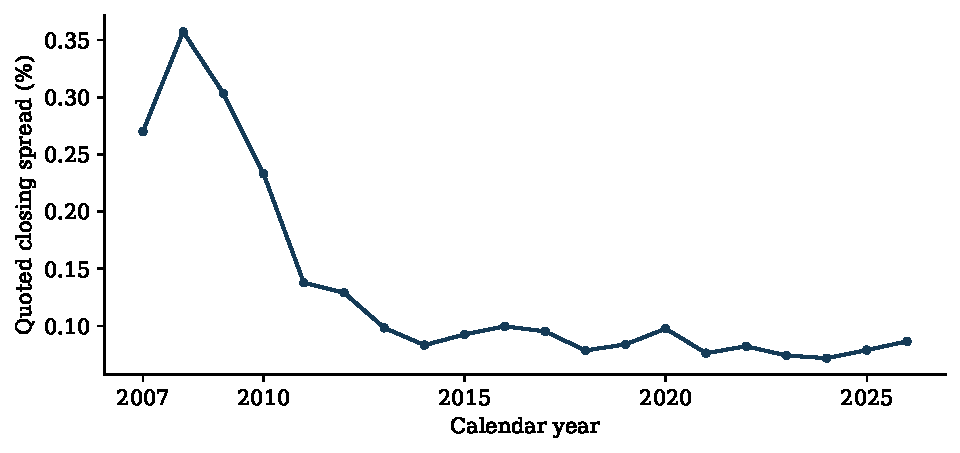
\includegraphics[width=.94\linewidth]{figures/quoted_spread.pdf}
\caption{Annual closing quoted spreads among OMXSB members. These vendor quote measures differ from the effective-spread and execution-cost evidence in Greenwood and Sammon.}
\label{fig:quoted_spread_appendix}
\end{figure}
\begin{figure}[!htbp]\centering
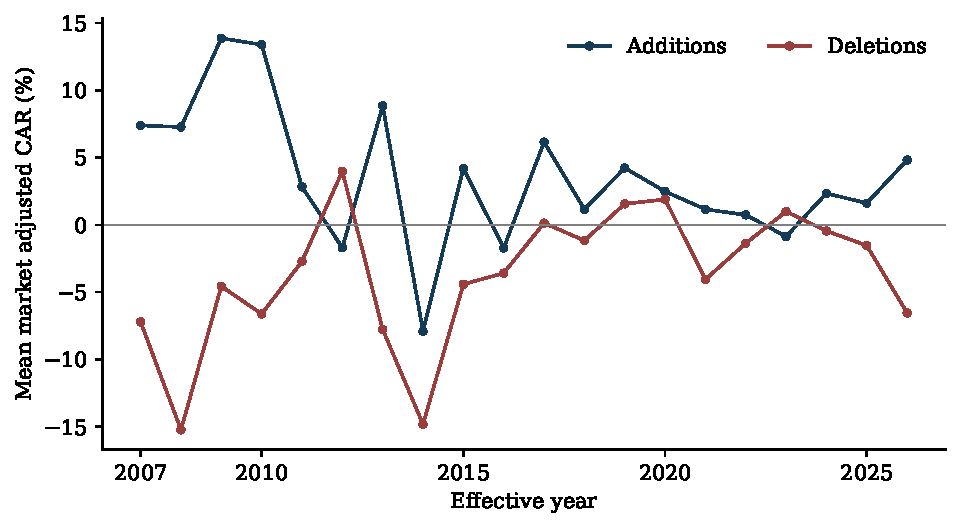
\includegraphics[width=.94\linewidth]{figures/annual_returns.pdf}
\caption{Annual event-return means. Annual averages describe the historical sample; sparse annual review counts limit their precision.}
\label{fig:annual_returns_appendix}
\end{figure}
\FloatBarrier

\section{Reproducibility and disclosure}
\label{app:audit}
\label{app:disclosure}

The analysis is anchored to repository commit \texttt{d2d41666ed21}, with the complete identifier and input hashes in the supporting manifest. Independent reconstruction verifies the main return arithmetic and selected estimators. Rerunning 40 numerical outputs reproduces point estimates and counts; eight differ in simulated inference. Some sparse auxiliary ratio intervals are unstable, so conclusions do not rely on those endpoints. These checks verify specified computations, not every source observation or identifying assumption.

The support package separates frozen estimates from repairs and exploratory additions, and records aggregate results, code, references and unresolved source checks. Licensed security-level data and third-party full texts are not newly redistributed. Reproduction requires authorized access to the documented inputs.

The paper's structure follows the six-part sequence in the BE451 course material. Earlier SSE theses by \citet{fager2024}, \citet{holst2023} and \citet{domeij2021} informed the emphasis on a focused question, a close benchmark study and self-contained exhibits. These examples were examined by Adrien d'Avernas; they are not evidence of an examiner-specific template for Riccardo Sabbatucci. The supporting structure note records the comparison.

\textbf{AI disclosure for this working document.} OpenAI Codex assisted with retrieval, calculations, code review, exhibits and manuscript composition; this prose is AI-generated. An earlier author-supplied draft prepared with Claude informed the narrative revision and was checked claim by claim against the sources and calculations. The BE451 syllabus permits disclosed assistance but prohibits AI directly writing thesis text \citep{sse2026}. This document is a research aid, not a submission-compliant manuscript. The authors must write the submitted prose, verify the findings and disclose assistance accurately.

\end{document}
